\chapter{Demonstration der Vorlage}
\label{sec:demo}
%
Dieser Abschnitt dient zur Demonstration der Vorlage. 


\section{Ein Kapitel}

Mit einer Formel
%
\begin{equation}
y = f(\vx) + w~.
\label{eq:formel}
\end{equation}
%
Das Symbol $\vx$ in \eqref{eq:formel} ist ein Vektor. 

Das \cite{Russell2009} ist der Verweis auf eine Literaturstelle. Tolles Buch. \Fig{fig:bild} kommt allerdings nicht in dem Buch vor.

\begin{figure}[b]%
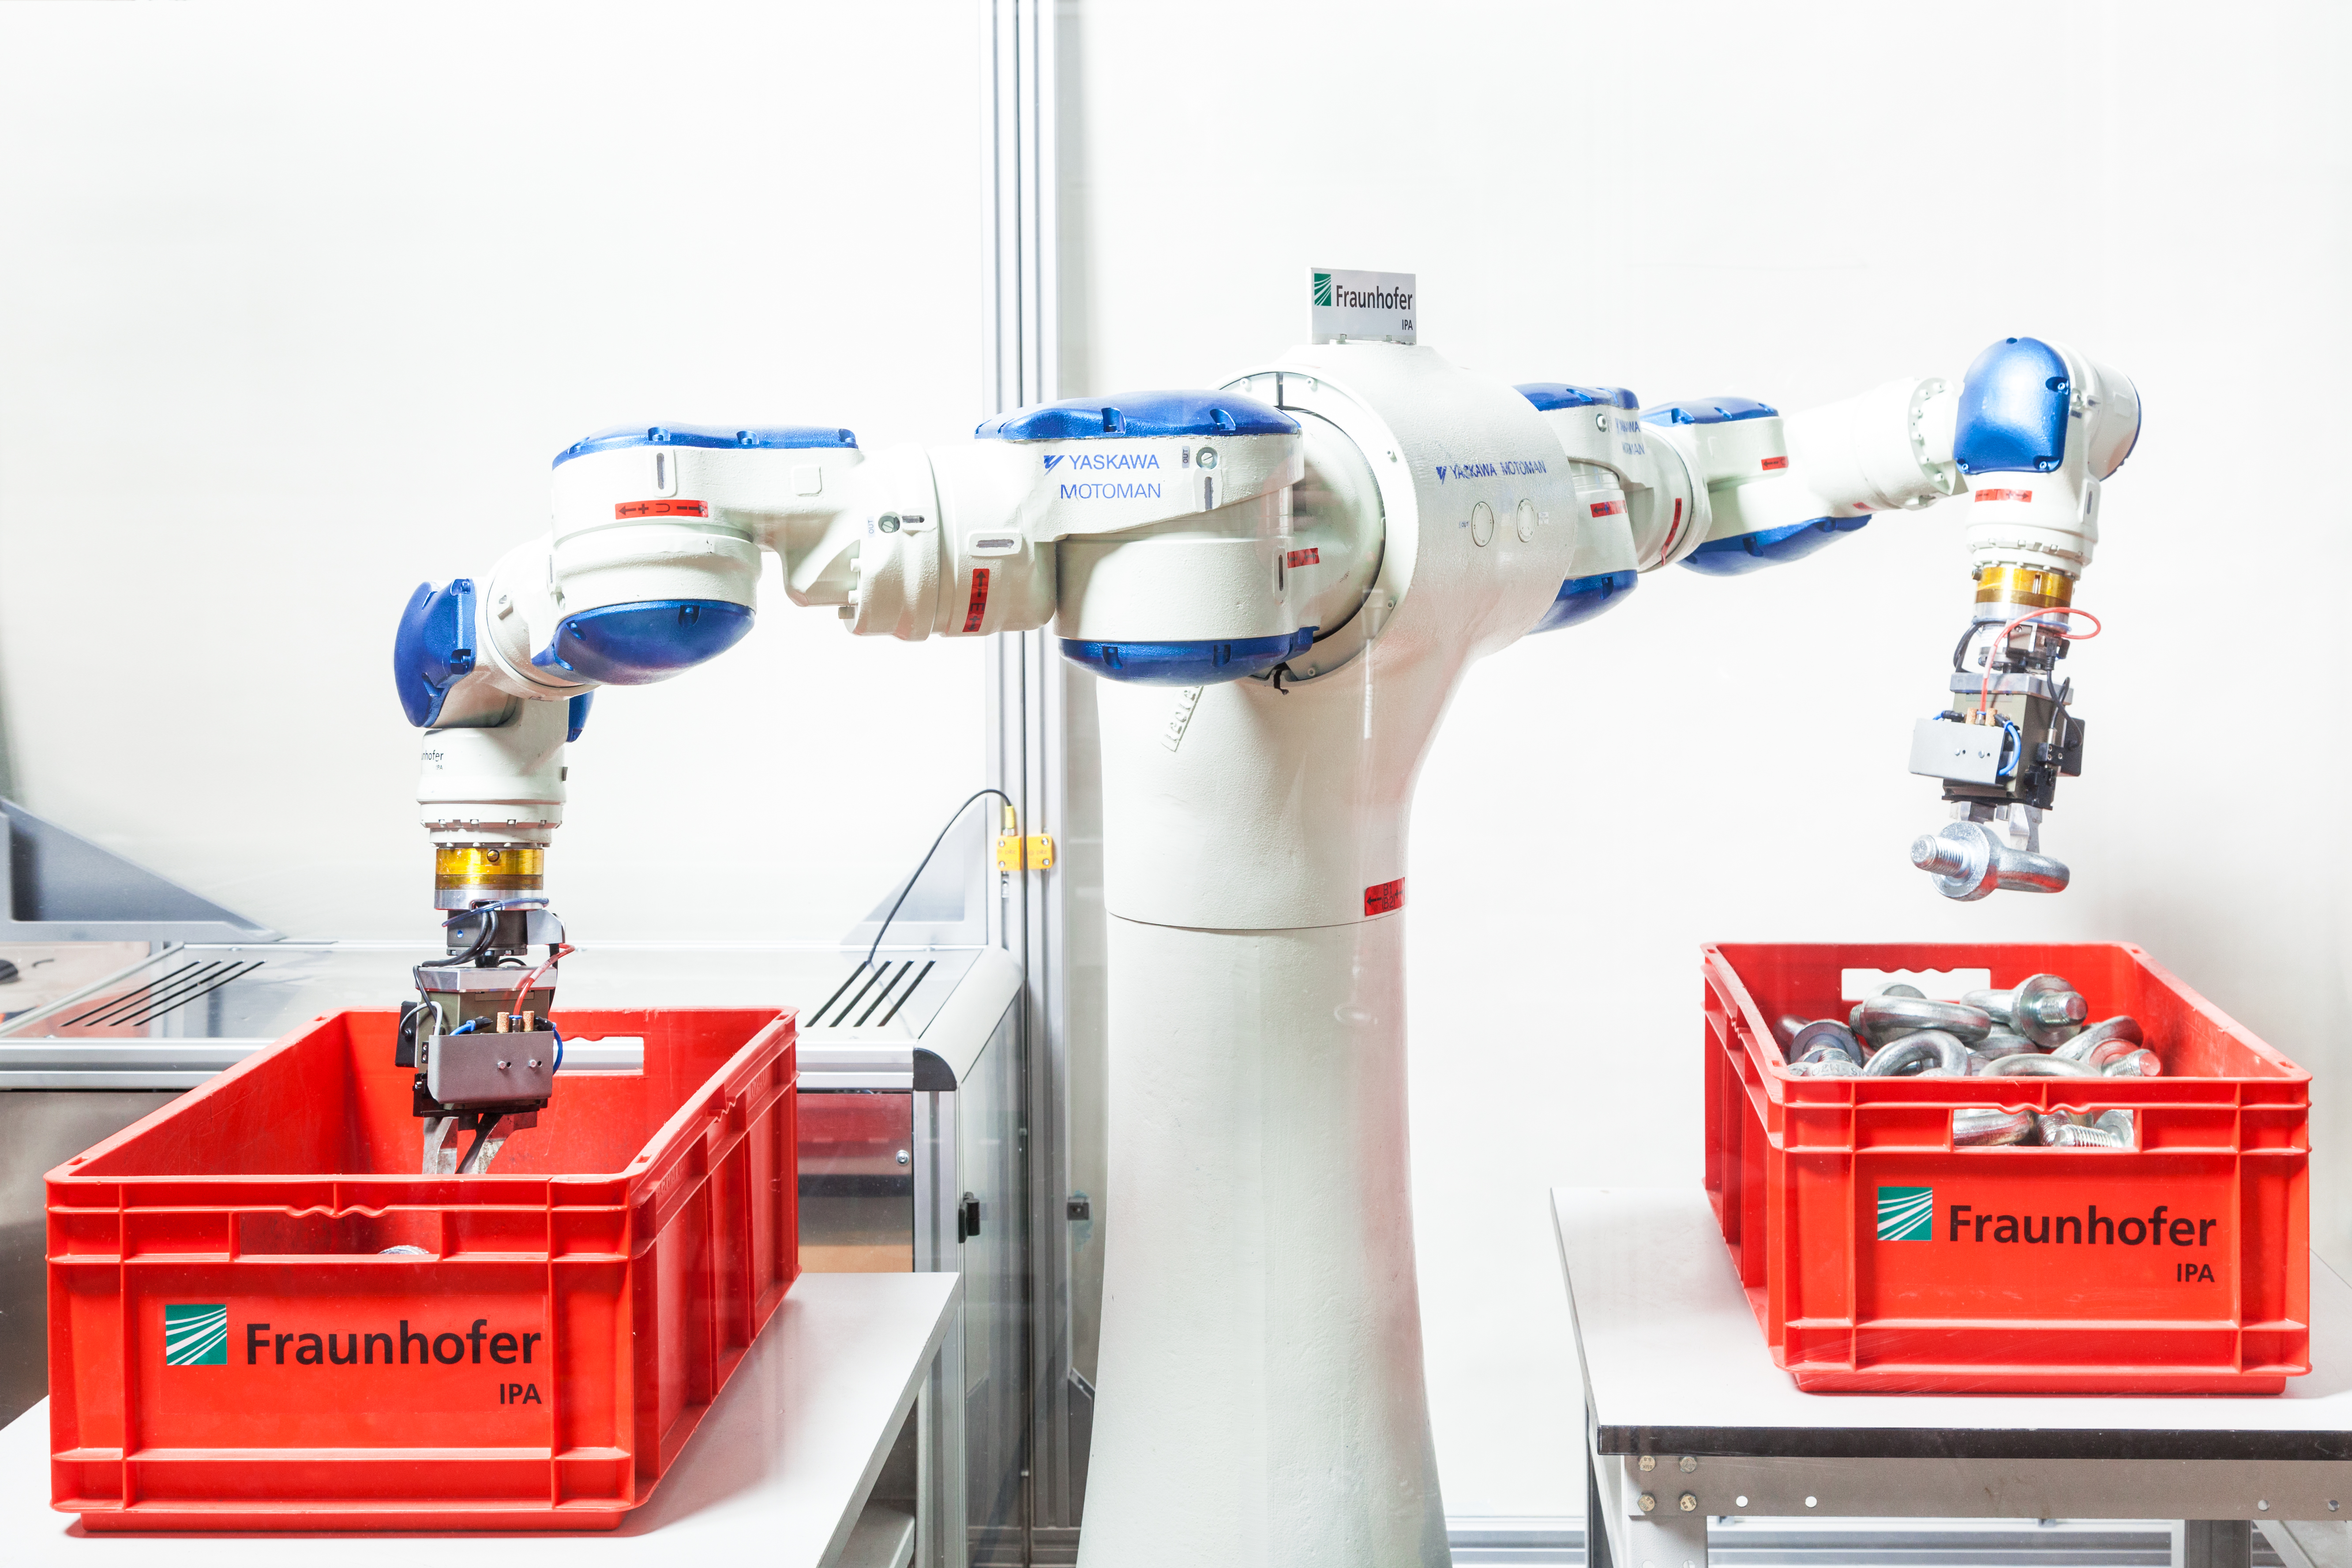
\includegraphics[width=\columnwidth]{Griff-in-die-Kiste}%
\caption{Griff in die Kiste.}%
\label{fig:bild}%
\end{figure}

Es gibt auch eine Beispielumgebung, wie man nachfolgend gut erkennen kann. Beispiel lassen sich mit \Ex{ex:beispiel} referenzieren. 

\begin{example}[Ein Beispiel]
\label{ex:beispiel}
Das ist die Beispielumgebung.
\end{example}

Auch Algorithmen lassen sich beschreiben und nat�rlich referenzieren mit \Alg{alg:algorithmus}.

\begin{algorithm}
\caption{Ein Algorithmus}
\label{alg:algorithmus}
\begin{algorithmic}[1]
\State Das ist eine Zeile des Algorithmus
\State Und das eine weitere Zeile
\end{algorithmic}
\end{algorithm}

Theoreme, S�tze, Lemmata, \usw gehen nat�rlich auch\footnote{Eine Fu�note}. Ziemlich beeindruckend diese Vorlage.

\begin{theorem}
Ein Theorem. Wird immer in kursiver Schrift dargestellt. 
\end{theorem}
\begin{proof}
Und der geht so...
\end{proof}

\todo{Das ist eine To-Do-Markierung}